\section{Taxonomy similarity}

In this section, we propose a new similarity to quantify the different kinds of relatedness of terms based on a taxonomy tree and propose the corresponding efficient string join algorithms.


\subsection{Similarity with taxonomy trees}


 We borrow the labeling scheme from XML databases and use the prefix based labels. Structural relationships between tree nodes whose positions
are recorded in this fashion can be determined easily for IS-A relationships.

\smallskip
\smallskip

\begin{definition}[Taxonomy Similarity]
Given two taxonomy tree nodes $n_1$ and $n_2$ with their prefix labels $L(n_1)$ and $L(n_2)$,  the similarity TS($n_1$,$n_2$) is the longest common prefix of  $n_1$ and $n_2$ over the length of the shorter path between $n_1$ and $n_2$, that is,  TS($n_1$,$n_2$,$\mathcal{T}$) = $\frac{|LCP(n_1,n_2)|}{|n_1|+|n_2|- |LCP(n_1,n_2)|}$. \end{definition}

\smallskip
\smallskip


\begin{example}
Consider Figure \ref{fig:taxonomyexample}, the similarity between ``\textsf{Seoul}'' (3.1.1.1) and ``\textsf{Suwon}'' (3.1.1.2) is $\frac{3}{5}$= 0.6 (as both countries are in South Korea.), and the the similarity between ``\textsf{Seoul}''  (3.1.1.1) and ``\textsf{Shenzhen}'' (3.2.1.1) is only $\frac{1}{7}$= 0.14 (as two countries are in Asia).
\end{example}

The complexity to computer TS is $O(|n_1|+|n_2|)$. This is efficient.


\subsection{ Nested-loop Join algorithms}


We would formulate the string similarity join problem and develop the corresponding algorithms. Given two collections of strings $S$ and $T$, a taxonomy tree
$\mathcal{T}$, and a similarity threshold $\theta$, a \textit{string
  similarity join} finds all string pairs $(s, t) \in S \times T$,
such that $TS(s,t,\mathcal{T})$ $>$ $\theta$, where \textit{TS} is
 the taxonomy similarity functions defined above.



Given two collections of strings $S$ and $T$, the baseline join algorithm is the nested-loop join. All string pairs are accessed to determine the IS-A relationships. But this algorithm is obviously not efficient. Therefore, we propose an efficient algorithm.

The complexity to computer the join set is $O(|S| \cdot |T| \cdot L^2)$, where L is the longest string in the set. This is not efficient.


\subsection{Indexed based join algorithms}

The first join method is based on the sort of data.

Associated with a collection $T$ there is a list $L_T$. This list contain the positional representation of the taxonomy tree nodes that match strings in the $T$. The nodes in the list are sorted by the lexicographical order. The operation over lists are: Eof, advance, next.
We main two cursors in each list: C1 and C2.

\begin{lem} Given a string $s$ with the length $|s|$, if any string t, $TS(s,t) > \theta$, then $s$ and $t$ share the prefix with the length of at least $|s| \cdot \theta $.
\end{lem}

The second join method is based on the taxonomy tree in the main memory.

\begin{figure}[t]
\centering
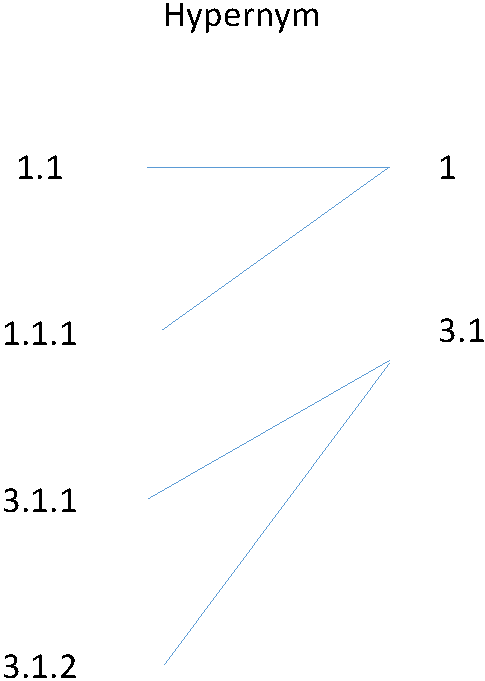
\includegraphics[scale=0.4]{figures/labeljoins}
 \caption{Join inverted lists}
\label{fig:invertedlist}
\end{figure}



\begin{algorithm}
{\bf Input}: two sorted lists of labels \\
{\bf Output}: string pairs $(s_1,s_2) \in L_1 \times L_2$, s.t. $TS(s_1, s_2) > \theta$
\begin{compactenum}[(1)]
\item Initialize  $C_1$, $C_2$ to point to the first elements in $L_1$ and $L_2$
\item {\bf WHILE}  $\neg$end($L_1$, $C_1$) and $\neg$end($L_2$,$C_1$) {\bf DO}
\item ~~ $L_{min}$ = the list with the smaller element and $L_{max}$ the larger
\item ~~ $p$ = prefix(cur($L_{min}$,$C_1$),$  \lceil l \cdot \theta \rceil$)
\item ~~ {\bf WHILE} (cur($L_{max}$,$C_2$) has the prefix $p$) {\bf DO}
\item ~~ ~~ ~~ {\bf IF} TS(cur($L_{max}$,$C_2$), cur($L_{min}$,$C_1$))$> \theta$ {\bf THEN}
\item ~~~   ~~ ~~ ~~ Add this pair to $R$
\item ~~ ~~ ~~  advance($L_{max}$,$C_2$)
\item $L_{max}.C_2$ =$L_{max}.C_1$
\item advance($L_{min}$,$C_1$)
\end{compactenum}
\caption{TS Join based on sorted labels}
\label{alg:exactjoin}
\end{algorithm}

The worst case complexity is $O(N^2)$, because the algorithm may compute each pair of strings with the prefix $p$. But this algorithm will skip many pairs of string for comparison. A theoretical analysis based on a random string model show that the average complexity is $O(\frac{N^2}{S^{\lfloor (1-\theta) \cdot l \rfloor}})$, where $N$ is the total number of elements in each list and $S$ is the maximal width of the taxonomy.


\begin{figure}[t]
\centering
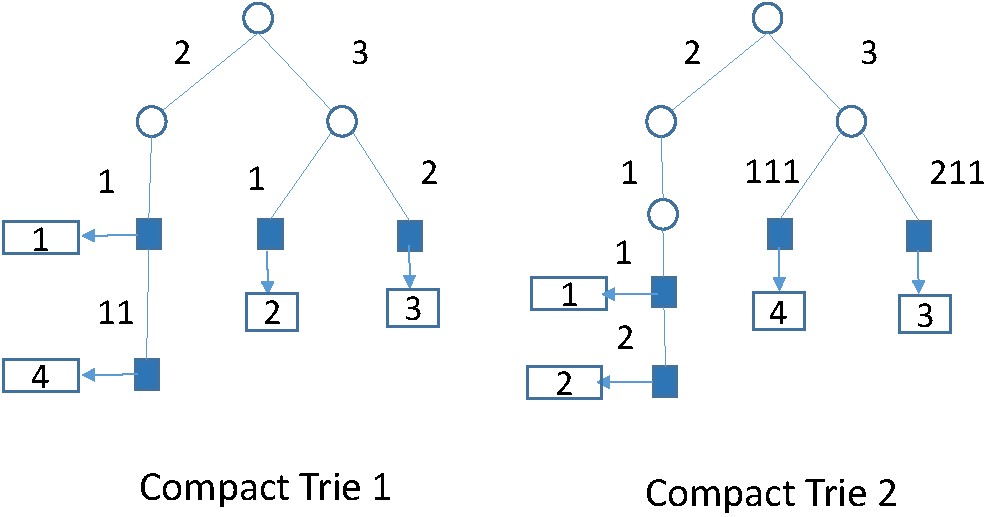
\includegraphics[width=0.35\textwidth]{figures/prefixTrees}
 \caption{An example of TS join based on prefix trees}
\label{fig:taxonomyexample}
\end{figure}


\begin{algorithm}
{\bf Input}: two sets of strings $S$ and $T$, a taxonomy $\mathcal{T}$, a threshold $\theta$ \\
{\bf Output}: string pairs $(s_1,s_2) \in S_1 \times S_2$, s.t. $TS(s_1, s_2) > \theta$
\begin{compactenum}[(1)]
\item Let $T_s$ and $T_t$ denote two prefix trees for $S$ and $T$ respectively.
\item {\bf WHILE} $\neg end(T_s) \vee \neg end(T_t)$ {\bf DO}
\item ~~ Let $T_{min}$ denotes the list with the smaller elements and $T_{max}$ is the larger 
\item  ~~ {\bf IF} ($T_{min}$ is a real element) {\bf THEN}
\item  ~~  ~~  Find($T_{max},T_{min}$)
\item ~~ {\bf ELSE IF} (isPotentialMatch($T_{min}$,$T_{max}$))  {\bf THEN}
 \item ~~~~ advance($T_{min}$)
 \item ~~~~~~~~~~~~~ {\bf ELSE} jump($T_{min}$)

\end{compactenum}
\caption{String joins with taxonomy}
\label{alg:exactjoin}
\end{algorithm}


\begin{algorithm}
{\bf Input}: A node n in $T_s$ and prefix $P$ of n in $T_s$ and a threshold $\theta$ \\
{\bf Output}:  pairs $R$ = \{$(n,m) \in L_1 \times L_2$ s.t. $TS(n,m) > \theta$\}
\begin{compactenum}[(1)]
\item FOR EACH i=1 to $|n|$
\item ~~~ $l$ = $\lceil \theta \cdot i \rceil$
\item ~~~ $p$ = $prefix(n,l)$
\item ~~~ IF $i < |n|$ AND $p \notin P$ THEN
\item ~~~~~~~ Add all nodes in $T_t$ with the length $i$ and the prefix $p$ to R;
\item ~~~ ELSE
\item ~~~  ~~~  Add all nodes in $T_t$ with the prefix $p$ to R;
\end{compactenum}
\caption{findTS(n,T,$\theta$)}
\label{alg:treejoin}
\end{algorithm}

\begin{lem} Given two strings $s$ and $t$,  assume that the $LCP(s,t) = x$. $TS(s,t) > \theta$ if and only if  $ x > \theta |s| $ and $  |t| < (\frac{1}{\theta}+1)x-|s|$.
\end{lem}
\begin{proof}  $TS(s,t) > \theta$ $\Leftrightarrow$ $\frac{x}{|s|+|t|-x} > \theta \Leftrightarrow |t| < (\frac{1}{\theta}+1)x-|s|$. In addition, note that $|t| \geq x$. Then $x < (\frac{1}{\theta}+1)x-|s|$ $\Rightarrow$ $x > \theta |s| $, which concludes the proof.
\end{proof}


In the findTS procedure, prefix(n,l) means to return the length-$l$-prefix of node $n$. For example, suppose $n$= 1.5.1.1,  prefix(n,3)=``1.5.1''.

\smallskip
\smallskip

\begin{example}
Consider the node Seoul  (3.1.1.1). Then $|n|$=4,
\end{example}

\smallskip
\smallskip


\begin{theorem}  Algorithm \ref{alg:exactjoin} is an optimal algorithm. The computing cost is linear to the sum of the size of the input and output. That is, each output result contribute to the final answer.
\end{theorem}




